\section{Preliminary results: Hohmann Transfer}

To validate the models created, a Hohmann transfer scenario is solved through direct optimization, and this solution is verified with primer vector theory and the known Hohmann transfer analytical solution.

The input orbital elements are given in table~\ref{tab:hohmann_orb_elems} and the orbits can be visualized in Figure~\ref{fig:hohmann_condition}. The blue dot is the initial position of the satellite and the yellow, its target position at the end of the control period. The lines represent the direction of the velocity.

\begin{table}[htbp]
    \centering
    \begin{tabular}{ccc} \toprule
        Element & Initial & Final \\ \midrule
        \(a\)      & \(7000km\)   & \(9000km\)   \\
        \(e\)      & \(0\)        & \(0\)        \\
        \(i\)      & \(51^\circ\) & \(51^\circ\) \\
        \(\Omega\) & \(0^\circ\)  & \(0^\circ\)  \\
        \(\omega\) & \(0^\circ\)  & \(0^\circ\)  \\
        \(\theta\) & \(0^\circ\)  & \(180^\circ\)  \\ \bottomrule
    \end{tabular}
    \caption{Orbital elements used for the Hohmann transfer case analysis}
    \label{tab:hohmann_orb_elems}
\end{table}

\begin{figure}[htbp]
    \centering
    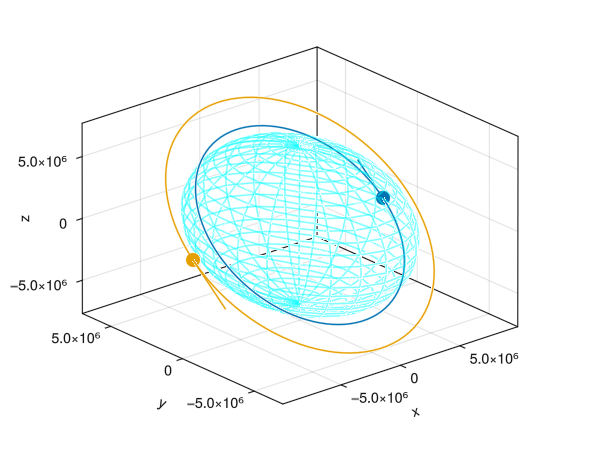
\includegraphics[width=0.6\textwidth]{img/hohmann_condition.png}
    \caption{Initial and final orbits for Hohmann transfer case visualization.}
    \label{fig:hohmann_condition}
\end{figure}

The total time was set to be equal to the analytical Hohmann transfer time\footnote{Methods for establishing how much time is needed for a certain maneuver shall be discussed in Future Results}, which from equation~\eqref{eq:hohmann_time} is calculated as \(t_f = 3560.54s\). Also from the analytical solution for the total change in velocity required, given in equation~\eqref{eq:hohmann_deltav}, \(\sum \lVert \Delta v \rVert = 887.56m/s\).

Initial guesses for \(\Delta t_1\) and \(\Delta t_2\) were arbitrarily proposed to be \(\frac{t_f}{3}\). The solution of the Lambert problem for the second coasting arc can be visualized in figure~\ref{fig:hohmann_lambert}. Naturally, this solution is very far from optimal but it is feasible, which is what is expected of it.

\begin{figure}[htbp]
    \centering
    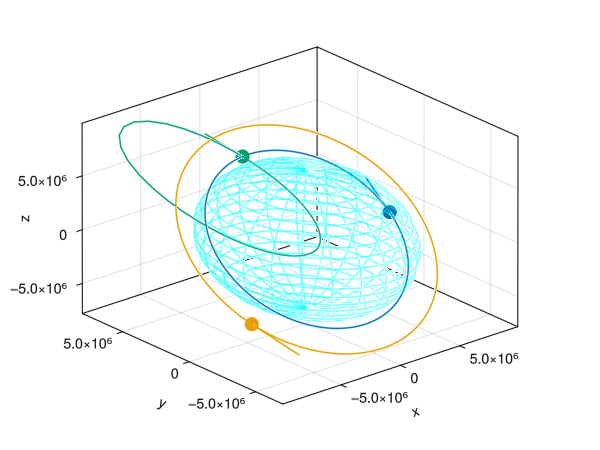
\includegraphics[width=0.6\textwidth]{img/hohmann_lambert_guess.png}
    \caption{Lambert problem solution for second coasting arc in Hohmann transfer case. This solution will serve as initial guess for the optimizer.}
    \label{fig:hohmann_lambert}
\end{figure}

Then, a discretization with \(N = 50\) was chosen. It was found that few steps lead to fast but imprecise solutions, which can often lead to infeasibility error conditions since the model is imprecise. Conversely, too many steps take much longer for no tangible gain in precision. The values of some variables are presented in table~\ref{tab:hohmann_results}, along with the expected analytical values. The solved, discretized trajectory can be seen in figure~\ref{fig:hohmann_traj}.

\begin{table}[htbp]
    \centering
    \begin{tabular}{ccc} \toprule
        Variable & Analytical & Solver \\ \midrule
        \(\Delta t_1\) & 0s & 8e-4s \\
        \(\Delta t_2\) & 3560.54s & 3560.538s \\
        \(\sum \lVert \Delta v \rVert\) & \(887.56m/s\) & \(887.56m/s\) \\ \bottomrule
    \end{tabular}
    \caption{Comparison of optimized and analytical values of some important variables in the Hohmann transfer case.}
    \label{tab:hohmann_results}
\end{table}

\begin{figure}[htbp]
    \centering
    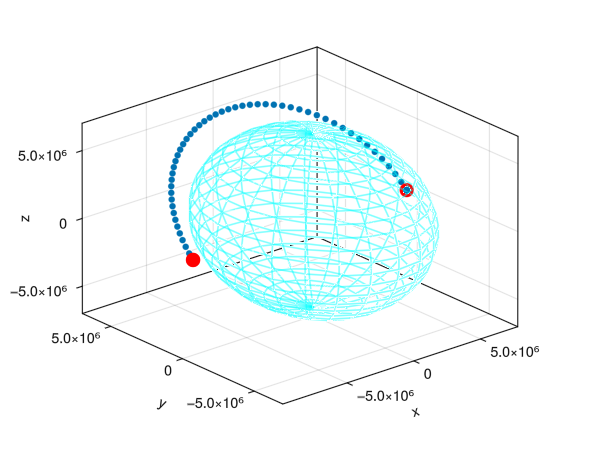
\includegraphics[width=0.6\textwidth]{img/hohmann_solved.png}
    \caption{Discretized transfer trajectory found by the numerical solver for the Hohmann transfer case.}
    \label{fig:hohmann_traj}
\end{figure}

Finally, primer vector theory is applied to verify is the found solution satisfies the optimality conditions. As a reminder, the number of impulses is not subjected to optimization and must be interactively changed based on primer vector trajectory results. The trajectory of the primer vector norm and its derivative are shown in figure~\ref{fig:hohmann_primer_vec}. The trajectory of the norm is continuous, and always less than 1, except for the impulse instants, when it has norm exactly one. Thus, the necessary conditions are satisfied and no modifications to the optimized trajectory can be extracted from the primer vector history.

\begin{figure}[htbp]
    \centering
    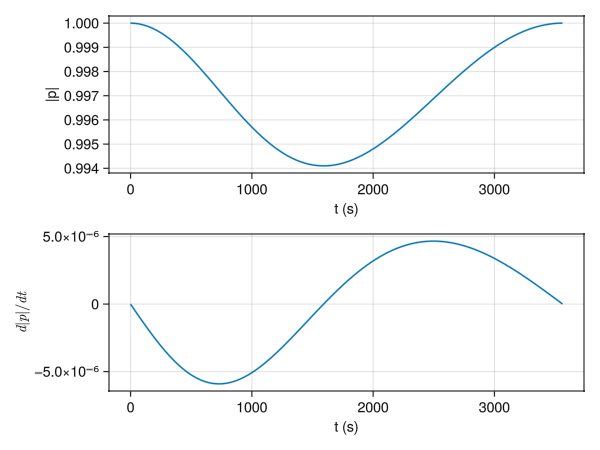
\includegraphics[width=0.6\textwidth]{img/hohmann_primer_vector_history.png}
    \caption{Primer vector norm and norm time-derivative trajectories for Hohmann transfer case.}
    \label{fig:hohmann_primer_vec}
\end{figure}

\section{Future results}